\begin{frame}{Layer 3 — Scan-ARE (1D-DBSCAN Segmentation)}
  \begin{columns}[T,onlytextwidth]
    \column{0.50\textwidth}
    \textbf{Idea.} Real-world keys are not uniform — they form clusters.
    \begin{itemize}
      \item One-pass 1D-DBSCAN over sorted keys, $O(n)$.
      \item \textbf{Dense} segments $\Rightarrow$ \textbf{exact} ERE \emph{(FPR = 0)}.
      \item \textbf{Sparse} regions $\Rightarrow$ truncation hash fallback.
    \end{itemize}
    \vspace{0.5em}
    \textbf{Density threshold:}
    \[
      \delta \;=\; c \cdot \mathcal{L}\,/\,\varepsilon
    \]
    No learning, no training data --- $\delta$ comes from the problem parameters.

    \column{0.48\textwidth}
    \centering
    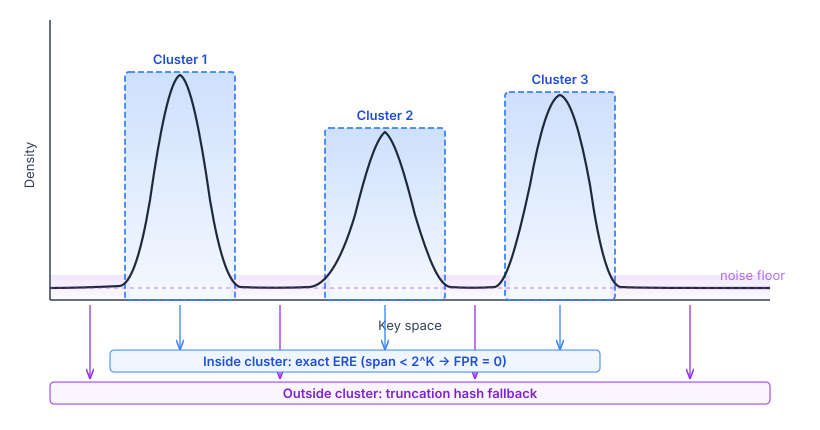
\includegraphics[width=\linewidth, keepaspectratio]{../../figures/segmentation.pdf}
  \end{columns}
\end{frame}
